\documentclass[aps,pra,reprint,amsmath,amssymb]{revtex4-1}

\usepackage{subfigure,dcolumn}
\usepackage[T2A,T1]{fontenc}
\usepackage[english]{babel}

\usepackage{braket}
\usepackage{graphicx}
\usepackage[colorinlistoftodos]{todonotes}
\usepackage[utf8]{inputenc}

% The following package will be used to typeset the LaTeX codes and is not a necessity to this template
\usepackage{listings}
\lstloadlanguages{[LaTeX]TeX}
\lstset{language=[LaTeX]TeX,keywordstyle=\color{red},showspaces=true,breaklines=true,breakatwhitespace=true,basicstyle=\small\tt,commentstyle=\color{white},frame=single,framerule=0pt,backgroundcolor=\color{yellow}}


\begin{document}


\title{Cluster principle + N-photon scattering matrix}

\author{...}
\affiliation{...}
\email[Corresponding author, ]{The name, complete address, telephone number, and e-mail address of the author to whom correspondence and proofs should be sent.}


\begin{abstract}
The scattering matrix is one of the most fundamental mathematical objects for particle processes. It connects the far past state with the far future state, where the particles are well described by a free Hamiltonian for both states, but they interact in some nontrivial way for mid times. It can always be split into two parts: the linear part, where each particle is scattered independently, and the nonlinear one, which gives information about the interaction among the particles. Here, we study the linear part of the scattering matrix for $N$ photons impinging on a local system with several stable states. 
\end{abstract}


\keywords{Quantum optics, scattering matrix, and few-photon photonics.}

\maketitle


\section{Introduction}

In the last years, a lot of effort has been devoted to the study of few photons interacting with few-level quantum systems \cite{fan10,Xu2015,Xu2016,Sanchez-Burillo2015,Sanchez-Burillo2016}

\begin{figure}
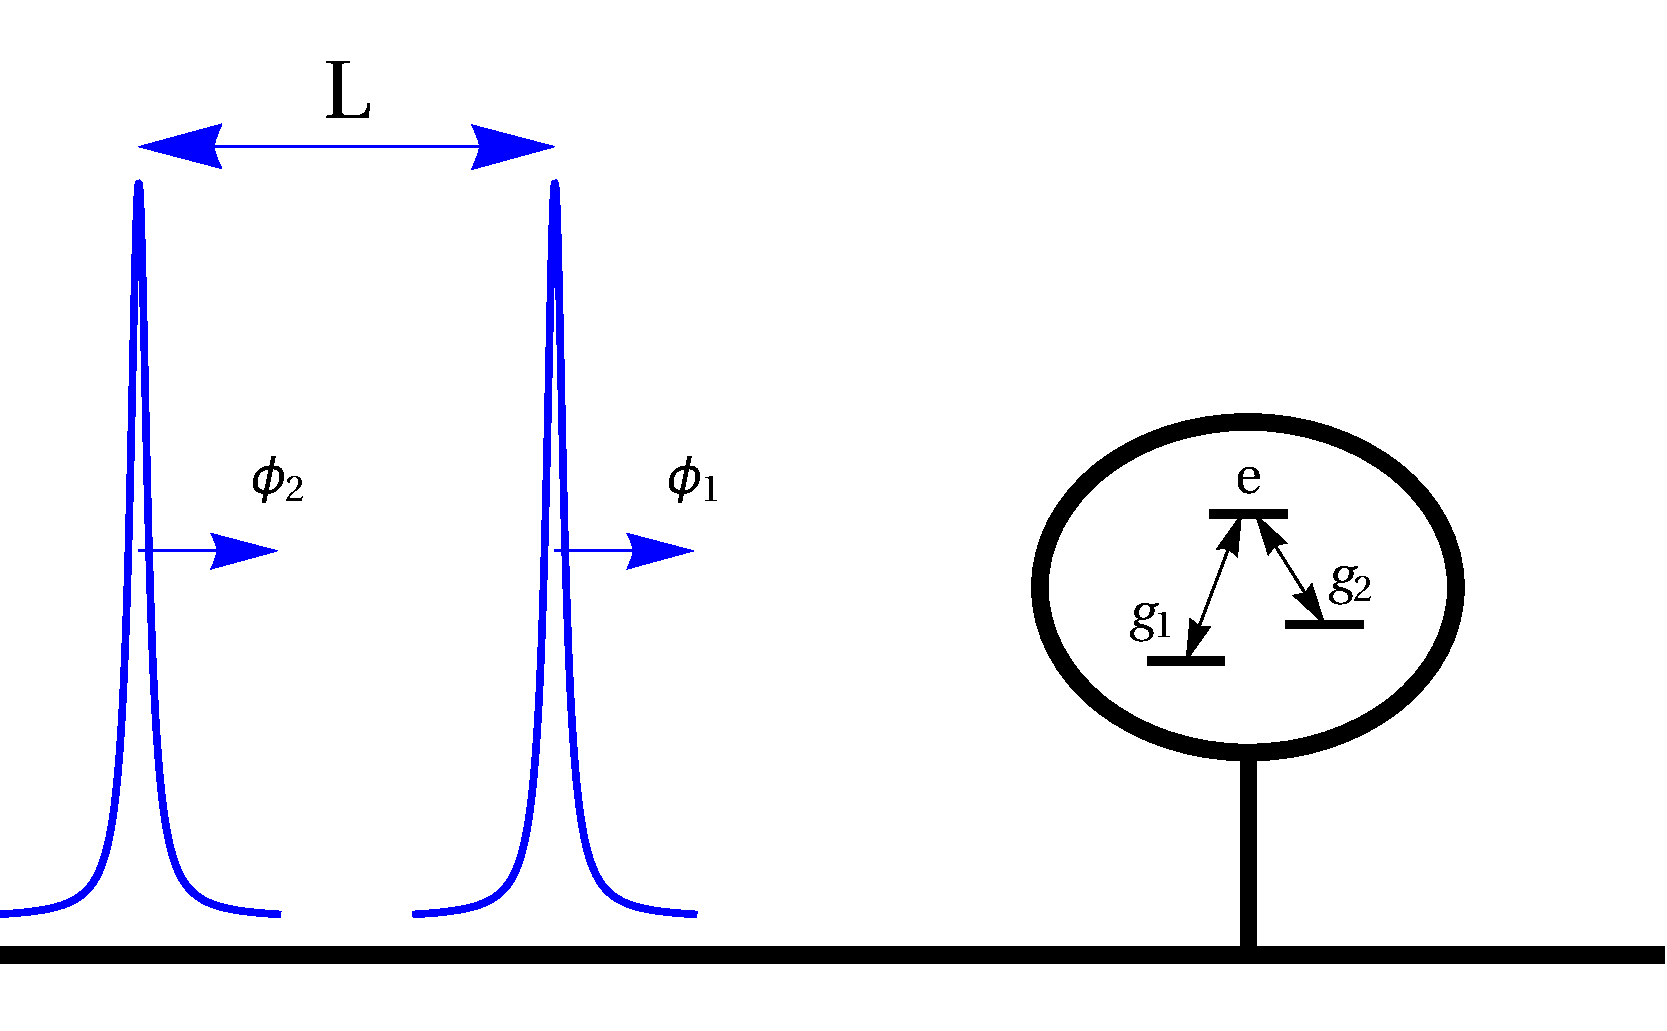
\includegraphics[scale=0.25]{input.pdf}
\caption{Two-photon input state impinging on a $\lambda$ atom.}
\end{figure}

\bibliographystyle{apsrev4-1}
\bibliography{bib_cluster}



\end{document}